\documentclass[10pt,conference,compsocconf]{IEEEtran}

\usepackage{hyperref}
\usepackage{graphicx}	% For figure environment


\begin{document}
\title{Machine Learning Project 1 : Higgs Boson Classification}

\author{
  Martin Cibils, Maxime Fellrath, Yura Tak, \\
  \textit{Department of Computer Science, EPFL, Switzerland}
}

\maketitle

\begin{abstract}
  In 2013, the discovery of Higgs boson is acknowledged by the Nobel prize in physics. With data provided by the ATLAS experiment at CERN, Higgs classification task became an interesting challenge. For this purpose, several machine learning models are tested. Our best model achieves 0.8 of accuracy.
\end{abstract}

\section{Introduction}

Higgs Boson, known to having the role of giving mass to other elementary particles, was discovered in 2012 in experiments at CERN. Using the ATLAS experiment data collected by CERN's particle accelerator, this project aims to predict whether an event was a Higgs boson or not. For this purpose, data preprocessing and hyperparameter tuning are done and various Machine Learning models are applied such as least squares, ridge regression and logistic regression. Each of these method's accuracy is estimated by applying cross-validation, then the model with highest accuracy is selected to actually perform the binary classification task. In the following section each of these steps are described.

\section{Data}
\label{sec:data}

Two datasets are provided: a training set with signal/background label and a test set without labels. Our machine learning models will be trained and cross-validated using the training set.

\subsection{Exploratory Data Analysis}
\begin{figure}[h]
  \centering
  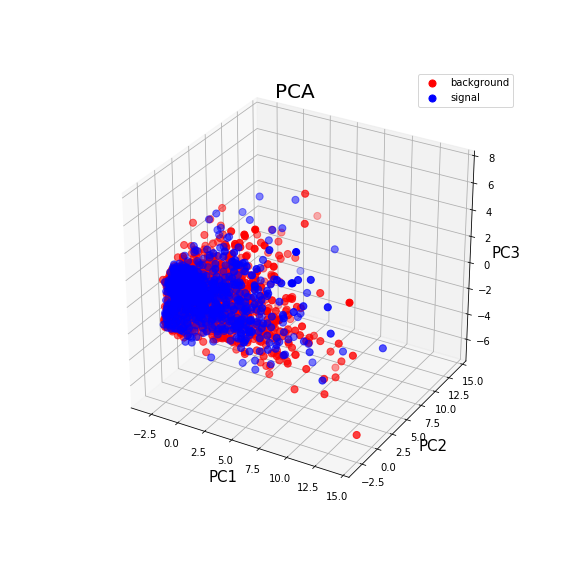
\includegraphics[width=2.5in]{pca.png}
  \caption{Visualization of the train data in 3D}
  \label{fig:pca}
\end{figure}

Each event is described with 30 features. We analyzed the data using PCA (Principle Component Analysis) method which is a mathematical technique used for dimensionality reduction. The Figure 1 is a visualization of the train data in 3-dimension.
By extracting 2/3 of the most relevant features, our accuracy dropped only by 3-4\% but the time for the training decreased significantly. However, we wanted to keep the optimal accuracy trading the running time for higher performance.

\subsection{Data Pre-processing}
Through our exploratory data analysis, we first learnt that there exists some undefined values having -999 as entry. Such undefined values are handled by replacing them by the median value of the corresponding feature where those undefined values aren't taken into account. Next step was detecting outliers: we used the IQR (Interquartile Ranges) method. Any values 1.5 IQR below 0-quantile and 1.5 IQR above 0.87-quantile were considered as outliers and removed. Final step was standardizing the data with respect to the training set mean and standard deviation.

The version of the logistic loss function we implemented needs labels to be 0 or 1, thus we modified the -1 data labels.

\section{Models and Methods}
\label{sec:model}

The following machine learning methods were implemented and tested:\\
Linear regression using gradient descent\\
Linear regression using stochastic gradient descent\\
Least squares regression using normal equations\\
Ridge regression using normal equations\\
Logistic regression using gradient descent\\
Regularized logistic regression using gradient descent\\




\subsection{Cross-Validation}
For an efficient use of the training data, we used 5-fold cross-validation. All the training data is used for the training and testing. Thereby the generalization error is estimated.

\subsection{Hyperparameter Tuning}
Grid search is used for the hyperparameter tuning such as gamma or lambda of different models. Each model would take different parameters from having none (ex: Least-Squares) to having up to three (ex: Regularized logistic regression with gamma, lambda and the degree). Moreover we also had the opportunity to use the Stochastic Gradient Descent which uses batches of size one in order to find the gradient. We decided to focus on the full Gradient Descent which makes the most of each data point but can take much longer to compute. The search range goes from 0 to 1. We also tuned the degree for least squares and ridge regression and degree 1 to 9 was tested. The accuracy severely dropped as we increased the degree of the expansion.
\begin{figure}[h]
  \centering
  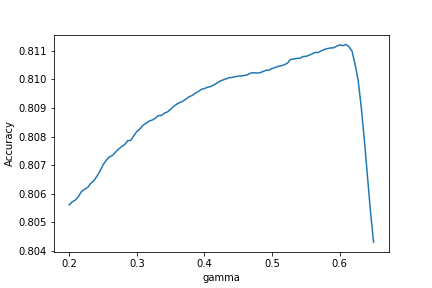
\includegraphics[width=3.1in]{graph.png}
  \caption{Example of grid search using Logistic regression and evaluating the accuracy w.r.t. the parameter gamma}
  \label{fig:pca}
\end{figure}
\subsection{Feature Augmentation}
As mentioned above, polynomial features have been concatenated to our original input data to augment our feature vector. Which means that using degree 2, our data looks like the following vector: $[1,X,X^2]$. In addition, different basis expansion has been tested with sin, log and exp functions. Thus despite of our linear model, using various feature augmentation, the underfitting is countered. 


\subsection{Model Selection}
We had different criteria in order to select the best model. The first one we used was the classic MSE. We would compute the weight for each method, do the cross-validation and thus get the MSE for both our training and our test set. As our problem here is a binary classification (either -1 and 1 or 0 and 1) the second criteria based on accuracy could indeed be more accurate. To do so, we would predict the label of each element of y be thresholding it: if it's above 0.5 we set it to 1, if it's lower we set it to 0. Finally we calculate the number of time our prediction is different from the final result. By doing so, we are not going to encounter any loss by doing the correct prediction unlike with a loss function such as the MSE or the L2 distance.\\


\subsection{Results}

As explained before, we valued our results according to the accuracy. The result is between 0 and 1, the closer we get to 1 the better our prediction. We've split our data in two set, one for the training and one for the testing with a ratio of 80\%\ of training and 20\%\ of testing. The results are available in the Table 1. The accuracy of the testing set seems to be more relevant as we didn't train our weight on them. We can see that the model that seems the most efficient is the logistic regression using a second degree polynomial expansion. With a very close result the model of Least Squares gradient descent also achieves some good results. It is making the most out of the Polynomial expansion by using a degree of 2. It is important to notice that we worked on 5 different folds and the result reported in the table are the average of each fold.\\

\begin{table}[h]
\resizebox{0.5\textwidth}{!}{%
 \begin{tabular}[c]{|c|c|c|c|c|c|}
    \hline
    Model Name&Accuracy Testing&Lambda&Gamma&Degree\\
    \hline
    Least Squares GD&0.781904&X&0.02&2 \\
    \hline
    Least Squares SGD&0.706140&X&0.001&2\\
    \hline
    Least Squares&0.717564&X&X&X\\
    \hline
    Ridge Regression&0.717564&0&X&X\\
    \hline
    Logistic Regression&\textbf{0.81118}&X&0.613636&2\\
    \hline
    Reg-logistic regression&0.81118&0&0.613636&2\\
    \hline
\end{tabular}%

}
    \caption{Finals results and finals parameters.}

\end{table}


\section{Discussion}
As we approached the classification problem methodically, our strength was to be able to observe the effects of each change on the results of our model as we appended them. However we did encounter strange or unexpected behaviors. For example, for Ridge regression and Regularized logistic regression the lambda parameters did not affect the accuracy, or if it did, it was negatively. This means we did not achieve to overfit our training set, even with high degree polynomial features expansion.
\section{Summary}
As we went on with this project, the accuracy we managed to improve followed a logistic growth, the further we got and the harder it was to gain the slightest edge. Because the logistic regression method obtained by far the best results in the beginning, it was the main method we tried to optimize. Even after many computationally expensive grid searches, this method always gave us the best results. This could mean that either the data was really well fitted for this model, or our data pre-processing was not good enough for the other ones. 

This Project was a great first experiment in the machine learning's world and was really helpful to understand the roots of it. Although we obtained satisfying results, we believe that in order to increase our test-accuracy we should try not only to improve our data pre-processing, but also try new methods such as SVM's, K-means or Neural Networks. 


\bibliographystyle{IEEEtran}

\end{document}
